\section{Workflow}\label{section:workflow}
% \todo{EB2DG: ``last two phases'' di cosa? Conviene ricordarlo, a meno che non sia banale. Quali sono le fasi?},
As we will see better in Chapter~\ref{chapter:use_cases} dedicated to practical use cases, where we will give more space to some technical details, 
my internship, for reasons of limited time and domain knowledge, has focused more on the last two phases, out of the four, of Zensor's product discussed previously in Section\ref{section:zensor_approach}. 
Now, in this last section, I would like to present some peculiar elements and techniques that Zensor employs for the 3rd and 4th phases: data management and analysis.

% https://www.notion.so/zensor/Scripting-Guidelines-8411d59eb62a454d8a5bea728f102bbb
\subsubsection{Architecture}
\begin{figure}[ht]
    \centering
    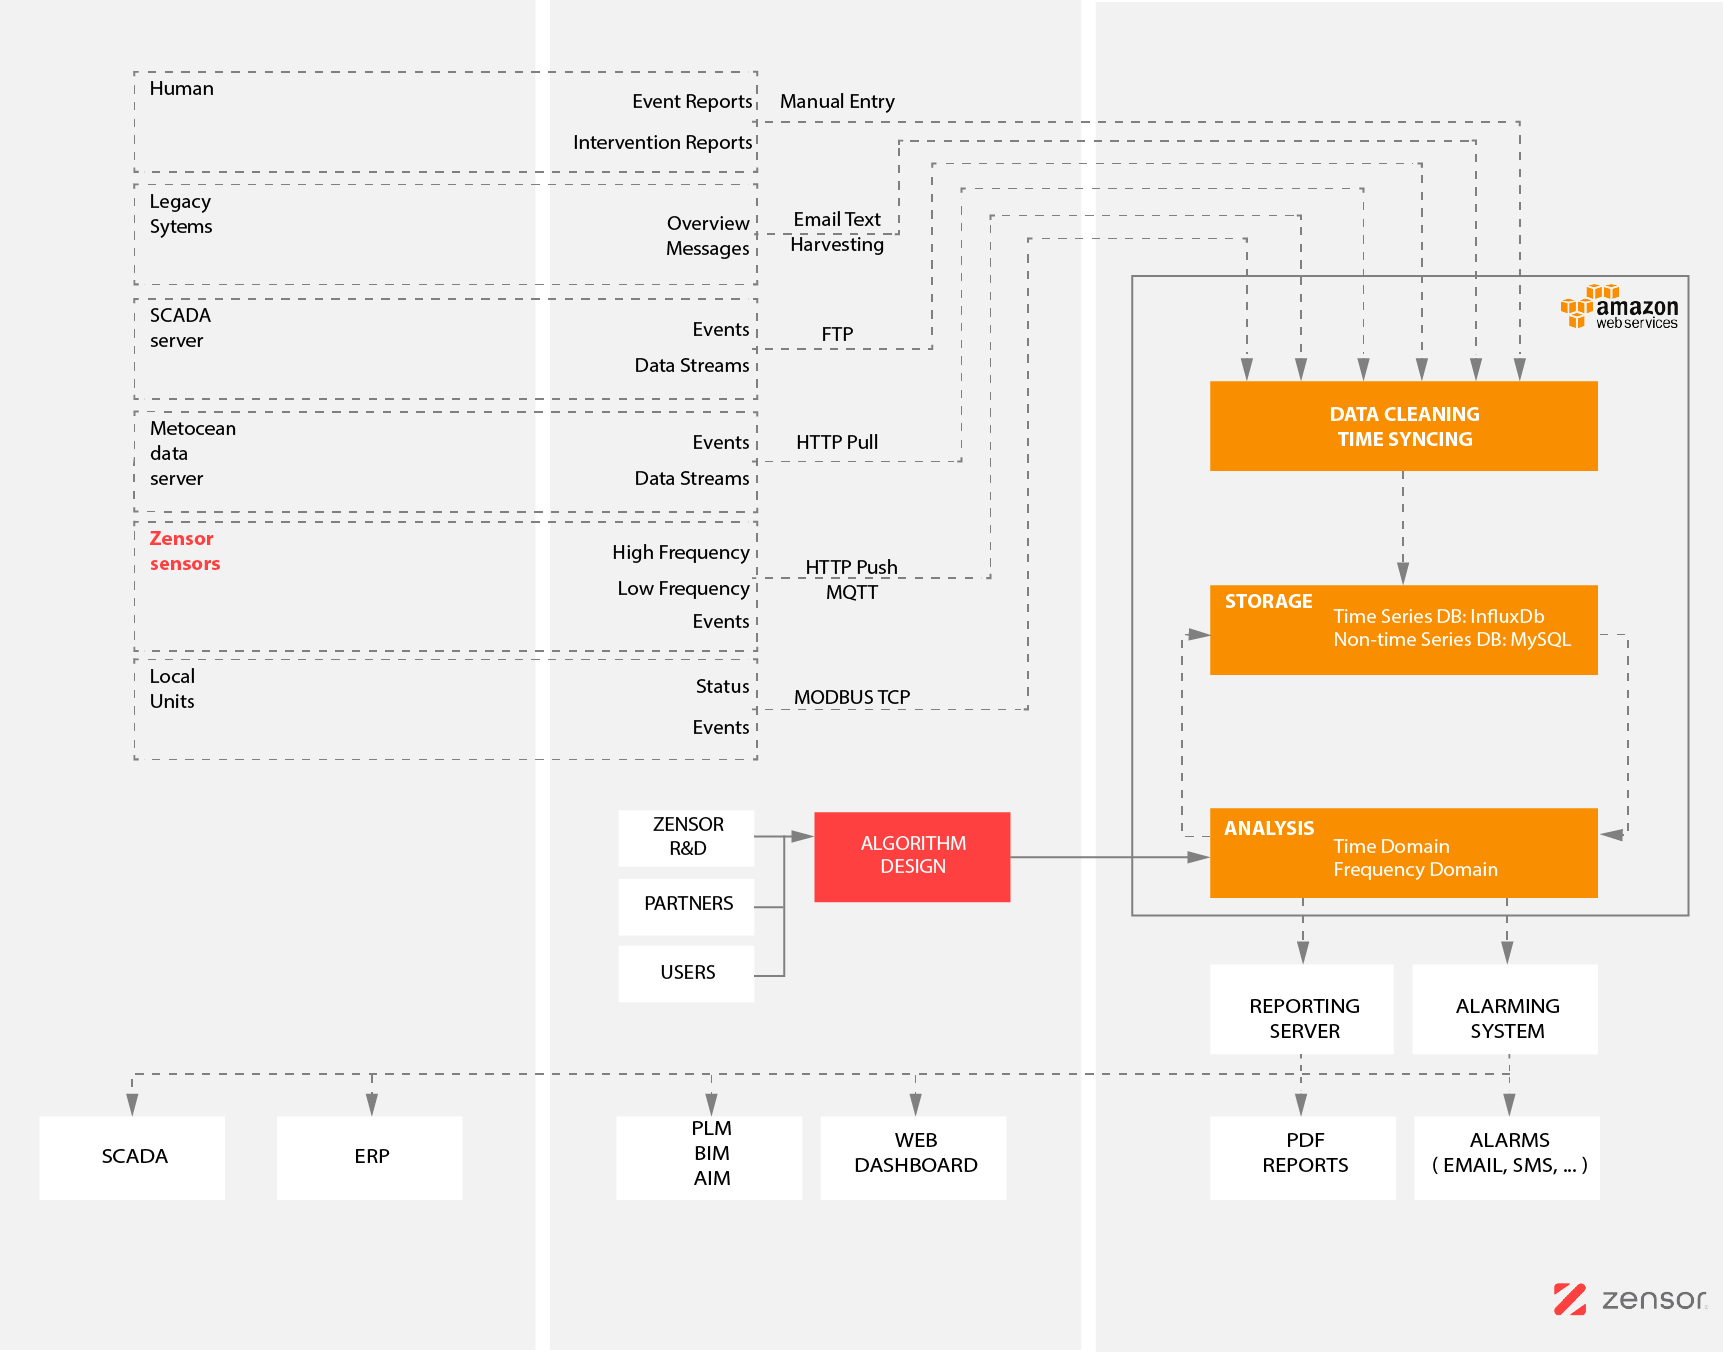
\includegraphics[width=\textwidth]{System_Architecture_Data Analytics.png}
    \caption{Zensor's system architecture for data analytics}
    \label{fig:zensor_sys_architecture}
\end{figure}
Assuming that the first two steps have gone well, we make a simplified scenario: the sensors of project \textit{22001\_XXX} have been properly installed and wired to the \acs{IPCs}, programmed by the engineering team to collect data and aggregate it into files. 
We could say that the ``pump'' from the data lake\footnote{Type of data repository that stores large and varied sets of raw data in its native format: \url{https://www.redhat.com/en/topics/data-storage/what-is-a-data-lake}} is up and running, but now the ``pipelines'' 
need to be built. As interesting a discussion as this is, this is likely to get off-topic. To stay at a shallow level let's look at Figure~\ref{fig:zensor_sys_architecture}; it shows us that:
\begin{itemize}
	\item The possible data sources, including our sensor data, are various, not to mention the formats or what protocols are used for managing transfer. 
	\item All ``roads'' lead to \textcolor{orange}{\ac{AWS}}, ensuring that each client will then have its own separate and independent cloud \textcolor{orange}{EC2}\footnote{Amazon Elastic Compute Cloud allows users to rent virtual computers on which to run their own computer applications.} 
	virtual machine, with its own domain.
		Once data reach this destination a sequence of operation may happen:\begin{enumerate}
		\item raw data gets cleaned, time synced and ingested in \textcolor{orange}{\ac{S3}}\footnote{AWS's Object-Storage service: it is not a file system, instead, is a 'Key-Value' store.} as backup system
		\item most of the continuous analysis, also designed and implemented by Zensor R\&D, is performed
		\item multiple services are running, like database and web dashboard instances, see InfluxDB \ref{section:influxdb} and Grafana \ref{section:grafana} respectively.
	\end{enumerate} 
	\item From there some advanced features are deployed: for instance an alarming system, with SMS and email notification, 
		or PDF reporting tool for ``freezing'' in time some of the most interesting dashboard panel with custom-made extra insights. %On top on this
\end{itemize}

% https://www.notion.so/zensor/Zensor-library-90259840e02349a7adc5cb2a48abf994
\subsubsection{Zensor Library}
Zensor library is an in-house developed Python package, containing functionality which is generic and useful to several projects. At present, the library contains the following main modules: 
clients, alerts and time.
\paragraph{Clients}
Influx client: easy interface to InfluxDB, built with the aid of Pandas~\ref{section:pandas}, for read/write operations from/to the database and for database management operations, like showing list of measurements or dropping a measurement.
Same goes from MySQL/Postgres client, that, at the moment of writing, has less functionality.
\paragraph{Alerts}
Three submodules are available:
\begin{itemize}
	\item Heartbeat: send a heartbeat (a lightweight daemon to periodically check the status of your services) from a server via the OpsGenie platform indicating that server and scripts docker are functioning well and are available.
	\item SMS: send an alert directly to list of phone numbers, with the downside that long messages will be cut off at 160 characters, but phone numbers aren't terribly format sensitive 
	and BE prefix +32 is automatically added, if no country code is specified.
	\item Email: This will send an E-mail through the \textcolor{orange}{AWS Simple E-mail service} where messages sent from EC2 instances are free up to 62,000 per month.
\end{itemize}
\paragraph{Time}
% \todo{EB2DG: controllare Inglese ``The contains''}
This includes two functions, designed to ease writing scripts that generate reproducible time ranges, ensuring that analysis is always aligned on the correct time window:
\begin{enumerate}
	\item[A] First one will generate evenly spaced timestamps in a given range.
	\item[B] The second one, instead generated pairs of times, which are separated by the argument (time) \texttt{interval}, the ``amplitude'' of the window.
\end{enumerate}
The goal of a good script should be that this happens reliably regardless of \textbf{when} exactly the script is run.
In this prospective, \textit{generate\_timewindow} can be useful e.g.\ to generate a window for the current year/month/week to date.

\subsubsection{Script Structure}\label{subsection:script_structure}
\begin{figure}
	\[\begin{tikzcd}
		&& Datasource \\
		&& {} \\
		Load && Process && Write
		\arrow[from=3-1, to=3-3]
		\arrow[from=3-3, to=3-5]
		\arrow[from=1-3, to=3-1]
		\arrow[from=3-5, to=1-3]
	\end{tikzcd}\]
	\caption{Analysis script structure}
	\label{tik:analysis_script}
\end{figure}

Most scripts that run on the Zensor platform have a very common structure~\ref{tik:analysis_script}, so for a given time window, they:
\begin{enumerate}
	\item Load batch of data (either raw or from InfluxDB).
	\item Process it in some (clever!) way, e.g.\ computing a derived metric.
	\item Write the results out to InfluxDB, to be shown in a dashboard.
\end{enumerate}
What time window they operate on will depend on what the task is, but also on whether the script is being invoked automatically by cron, a job scheduler on Unix-like OS, or manually.
If a script is being invoked \textit{manually}, this is usually to run it over historical data (e.g.\ rerunning a script for the month of February 2022). We typically call this operation \textbf{backfilling}.
Typically, if the script is running in \textit{cron}, it's loading ``recent'' data (e.g.\ from the past hour or past day) ending at the time the script started.
Scripts on the Zensor platform need to support running in both modes, so there are a few guidelines to keep in mind when writing code.
